\section*{Elméleti kérdések kidolgozása}
	
\subsection{ Írd fel egy exportált rutin és egy exportált creation procedure szerződését Hoare-hármasok segítségével, és magyarázd el a különbséget! }

	Az alapvető különbség, hogy egy $r$ rutin megőrzi az osztály invariánst, míg a creation procedure-nek (természetesen) csak az utófeltételében szerepel. Tehát,
	\begin{align*}
	\{Q_m\}\quad&make \quad\{inv_C\wedge R_m\} \\
	\{inv_C\wedge Q_r\} \quad&r\qquad\quad\{inv_C\wedge R_r\},
	\end{align*}
	ahol $r$ az exportált rutin, $make$ az exportált creation procedure és $inv_C$ az osztály invariánsa. Emellett $Q_r$ és $R_r$ az $r$ rutin, míg $Q_m$ és $R_m$ a creation procedure elő- és utófeltétele.


\subsection{ Mi a szerepe a \lstinline[language=Eiffel]|like| kulcsszónak az Eiffelben? }\label{like}

	Öröklődési hierarchiában sokszor okozhat gondot, ha egy típust az alosztályok megfelelő közös ősével szeretnénk meghatározni. Az öröklődés és polimorfizmus miatt Objektum-orientált nyelveknél sok esetben fordulhat elő az az eset, hogy nem ismerjük az egyes változók dinamikus típusát fordítási időben. Ez az ismeret viszont sok esetben fontos lenne. Például a Java-ban az \lstinline[language=Java]|equals| függvény az \lstinline[language=Java]|Object| osztályon definiálva a következő szignatúrával rendelkezik,
	\begin{lstlisting}[language=Java]
	public boolean equals(Object obj)
	\end{lstlisting}
	
	Ebben az esetben egy \lstinline[language=Java]|String| típusú objektumra bármikor meg lehet hívni az \lstinline[language=Java]|equals| függvényt bármely \lstinline[language=Java]|Object|-ből származó paraméterrel (pl. \lstinline[language=Java]|Integer|)
	
	Az Eiffelben ennek a jelenségnek a kiküszöbölésére vezették be a \lstinline[language=Eiffel]|like| kulcsszót, mellyel ún. \textit{kapcsolt típusokat} (anchored type) lehet létrehozni. Ezt a kulcsszót többféleképpen is lehet használni. Az előző példában látható jelenség elkerüléséhez a következő szignatúrát írhatjuk Eiffelben,
	\begin{lstlisting}[language=Eiffel]
	is_equal (other: like Current): BOOLEAN
	\end{lstlisting}
	A \lstinline[language=Eiffel]|Current| az aktuális osztály típusára hivatkozik, így bármely leszármazotton a megfelelő paramétertípussal fog rendelkezni a függvény.
	
	Az osztály típusa mellett hivatkozhatunk azonosító típusára is, így növelve a kód újrafelhasználhatóságát.
	\begin{lstlisting}[language=Eiffel]
	like <azonosito>
	\end{lstlisting}
	
	 Tekintsünk egy egyszerű példát, ahol síelő fiúkat és lányokat akarunk elszállásolni, viszont csak az azonos neműeket szeretnénk egy szobába tenni. Ezt a típusokkal tudjuk elérni a következő módon.
	\begin{lstlisting}[language=Eiffel]
	class SKIER
	feature
		roommate: like Current
		
		share( other: like roommate ) is
		require
			other /= Void
		do
			roommate := other
		ensure
			other = roommate
		end
	end
	\end{lstlisting}
	Láthatjuk, hogy a \lstinline[language=Eiffel]|roomate| attribútum típusa \lstinline[language=Eiffel]|like Current| azaz meg kell egyezzen az aktuális típussal (A \lstinline[language=Eiffel]|Current| az aktuális objektumot jelöli. Olyan, mint Java-ban a \lstinline[language=Java]|this|.). Ez azt jelenti, hogy ha egy \lstinline[language=Eiffel]|GIRL| osztályt leszármaztatunk a \lstinline[language=Eiffel]|SKIER| osztályból, akkor annak a \lstinline[language=Eiffel]|roomate| attribútumoka is \lstinline[language=Eiffel]|GIRL| típusú kell legyen. Emellett láthatjuk, hogy a \lstinline[language=Eiffel]|share| metódus paramétere \lstinline[language=Eiffel]|like roomate| típusú, magyarul csak olyan objektumot adhatunk paraméterként, mely megegyezik a \lstinline[language=Eiffel]|roomate| típusával. (\lstinline[language=Eiffel]|GIRL| esetén csak \lstinline[language=Eiffel]|GIRL| lehet)
	
	Megjegyzés: Létezik kiskapu, van lehetőségünk fiúkat és lányokat egy szobába rakni. Ezt a kiskaput "Polymorphic CAT-call"-nak hívják.
	
	Az \lstinline[language=Eiffel]|ANY| osztálynak van egy \lstinline[language=Eiffel]|copy| feature-e, melyet a következőképpen definiált,
	\begin{lstlisting}[language=Eiffel]
	copy (other: like Current)
	\end{lstlisting}
	
\subsection{ Mi a mixin-inheritance lényege? }\label{Mixin}
	Mixin-inheritance amikor egy generikus paraméterből származtatunk le. 
	\begin{lstlisting}[language=C++]
	template <class Base>
	class Mixin : public Base  { ... };
	
	class Base { ... };
	\end{lstlisting}
	A többszörös öröklődés által okozott kétértelműséget hivatott kiküszöbölni. A mixin-ek linearizálják az öröklést, így oldják fel a problémákat. Különböző nyelvek különbözőképpen alkalmazzák.
	
	
	Például C++ esetében,
	\begin{lstlisting}[language=C++]
	template <typename T> class Numeric : public T { ... };
	template <typename T> class Comparable : public T { ... };
	class Base {};
	\end{lstlisting}
	Ekkor a következő módon lehet \lstinline[language=C++]|Rational| osztályt definiálni,
	\begin{lstlisting}[language=C++]
	class Rational : Comparable< Numeric<Base> > { ... };
	\end{lstlisting}
	
	Eiffel-ben nem lehetséges mixin-ek definiálása.

\subsection{ Milyen szerződések vonatkoznak az Eiffel rutinokra? Hogyan befolyásolja ezt az öröklődés? Hogyan a felüldefiniálás? Magyarázd el a kapcsolódó fogalmakat és szabályokat. Fogalmazd meg a szerződéseket Hoare-hármasok segítségével! }\label{öröklődés}
	Eiffelben a rutinokra explicit módon az elő- és utófeltétel szerződések vonatkoznak, míg implicit módon az osztály invariáns.
	\begin{align*}
	\{Q_r \wedge inv_C\} r \{R_r \wedge inv_C\},
	\end{align*}
	ahol $Q_r$ és $R_R$ az $r$ elő- és utófeltételei, míg $inv_C$ az osztály invariánsa.
	
	Az öröklődés és polimorfizmus talán legnagyobb kérdése a \textit{variancia}. A variancia két típus helyettesíthetőségét fejezi ki. $A :> B$ az altípus relációt jelenti, vagyis ebben az esetben a $B$ típus az $A$-nak altípusa.
	
	\textit{Kovarianciának} nevezzük, ha az általánosabb $A$ típus helyére a speciálisabb $B$ típust behelyettesíthetjük.
	
	\textit{Kontravarianciának} nevezzük, ha a speciálisabb $B$ típus helyére az általánosabb $A$ típust helyettesíthetjük be.
	
	\textit{Invariáns} vagy \textit{nonvariáns} a reláció, ha a fentiek közül egyik sem mondható.
	
	A fent említett tulajdonságok kontextustól függőek. A legfontosabb felhasználási területe ezeknek a tulajdonságoknak az öröklődés során a metódusok specializációja. Egy metódust akkor tudunk típushelyesen specializálni, ha a paraméterei kontravariánsak az ősosztály metódusának paramétereivel, míg a visszatérési típusa kovariáns a ősosztály metódusának visszatérési típusával.
	
	Tekintsük a következő példát! Tegyük fel, hogy $ CREATURE :> ANIMAL :> MONKEY$ és $FOOD :> FRUIT :> BANANA$, illetve létezik egy \lstinline[language=Eiffel]|ANIMAL_FEEDER| osztályunk,
	\begin{lstlisting}[language=Eiffel]
	class ANIMAL_FEEDER 
	creation
		make
	feature {ANY}
		feed(a : ANIMAL) : FRUIT
		do 
			-- implementation
		end
	end
	\end{lstlisting}
	Ha létre akarjuk hozni a \lstinline[language=Eiffel]|MY_FEEDER| osztályt és specializálni szeretnénk a \lstinline[language=Eiffel]|feed| metódust, akkor a paramétere lehet továbbra is\lstinline[language=Eiffel]| ANIMAL| típusú, vagy \lstinline[language=Eiffel]|CREATURE|, de \lstinline[language=Eiffel]|MONKEY| semmiképp. Ugyanis azon a helyen, ahol kicseréljük az \lstinline[language=Eiffel]|ANIMAL_FEEDER| példányt, az azt használók nem feltétlenül csak \lstinline[language=Eiffel]|MONKEY| típusú paramétereket adhatnak át. Hasonlóképpen a visszatérési érték csak \lstinline[language=Eiffel]|FRUIT| és \lstinline[language=Eiffel]|BANANA| lehet. Az \lstinline[language=Eiffel]|ANIMAL_FEEDER|-t használók \lstinline[language=Eiffel]|FRUIT| típust vagy annak altípusait várják értékül.
	
	Ahogy a metódusok paramétereire és visszatérési értékére, a szerződésekre is érvényes a variancia. A feature-ök előfeltételeit lazítani lehet, míg az utófeltételeit megszorítani. Erre a \lstinline[language=Eiffel]|require else| és \lstinline[language=Eiffel]|ensure then| kulcsszavakat lehet használni. A \lstinline[language=Eiffel]|require else| esetén az újonnan megfogalmazott előfeltétel \textit{vagy} kapcsolatban fog állni az eredetivel. Az \lstinline[language=Eiffel]|ensure then| esetén az utófeltétel szigorodik, \textit{és} kapcsolatban fog állni az eredeti utófeltétellel.
	Tehát, ha $B <: A$, akkor $B$ minden $r$ rutinjára teljesülnie kell a következőnek
	\begin{align*}
	\{Q_{rA} \vee Q_{rB}\} r \{R_{rA} \wedge R_{rB}\}
	\end{align*}	
	
	Az öröklődés során Eiffelben a leszármazottak megőrzik az ősök osztályinvariánsait. Így a leszármazott invariánsa a leszármazottban megfogalmazott invariáns és ősei invariánsának konjunkciója lesz (össze\textit{és}elődnek).
	Tehát, ha $B <: A $, akkor $B$ minden $r$ rutinjára a következő teljesül
	\begin{align*}
	\{Q_r \wedge inv_A \wedge inv_B\} r \{R_r \wedge inv_A \wedge inv_B\},
	\end{align*}
	ahol $Q$ és $R$ az $r$ elő- és utófeltételei, míg $inv_j$ a megfelelő $j$ osztályok invariánsai.

\subsection{ Milyen viszonyban kell álljanak az $A_i$ és a $B_j$ típusok ahhoz, hogy fennálljon az alábbi altípus reláció (matematikailag helyesen)? Indokold válaszod! $(A_1 \rightarrow A_2) \rightarrow A_3 \rightarrow A_4 <: (B_1 \rightarrow B_2) \rightarrow B_3 \rightarrow B_4$ }

	Az elhagyott zárójeleket kitéve a kifejezés a következő
	\begin{align*}
	((A_1 \rightarrow A_2) \rightarrow (A_3 \rightarrow A_4)) <: ((B_1 \rightarrow B_2) \rightarrow (B_3 \rightarrow B_4)).
	\end{align*}
	A paraméter kontravariáns, az eredmény kovariáns kell legyen, így
	\begin{align*}
	( B_1 \rightarrow B_2 ) &<: ( A_1 \rightarrow A_2) &
	( A_3 \rightarrow A_4 ) &<: ( B_3 \rightarrow B_4).
	\end{align*}
	Ugyanezen gondolatmenet alapján,
	\begin{align*}
	A_1 &<: B_1,& B_2 &<: A_2,& B_3 &<: A_3,& A_4 &<: B_4.
	\end{align*}

\subsection{ A strukturális altípusosságot hogyan szokás definiálni direktszorzat (tuple) típusokra? }
	Általánosságban a kovariancia jellemző, vagyis
	\begin{align*}
	TUPLE[INTEGER,STRING]&<:TUPLE[INTEGER,ANY]<:\\&
	 <:TUPLE[INTEGER]<:TUPLE[ANY]<:TUPLE.
	\end{align*}


\subsection{ A strukturális altípusosságot hogyan szokás definiálni rekord típusokra? }
	Általánosságban a kovariancia jellemző, vagyis
	\begin{align*}
	\{x_1:\sigma_1,\cdots,x_n:\sigma_n,\cdots,x_m:\sigma_m\}<:\{x_1:\sigma_1,\cdots,x_n:\sigma_n\}
	\end{align*}

\subsection{ Mire való az old kulcsszó az Eiffelben? Magyarázd el, fogalmazd meg a rá vonatkozó szabályokat, illusztráld használatát példán! }\label{old}
	Eiffelben az \lstinline[language=Eiffel]|old| kulcsszót utófeltételekben szokás használni. Egy azonosító régi értékére lehet vele hivatkozni. Tegyük fel, hogy \verb|x| az osztály egy attribútuma. Ekkor megfogalmazhatjuk a következő feature-t.
	\begin{lstlisting}[language=Eiffel]
	increment
	do
		x := x + 1
	ensure
		x = old x + 1
	end
	\end{lstlisting}

\subsection{ Hogyan működik, miért és mire jó az átnevezés az öröklődés során? }\label{atnevezes}
	Többszörös öröklődés esetén az ősosztályokban lévő megegyező nevű feature-öket átnevezéssel tudjuk megkülönböztetni egymástól.

\subsection{ Mit jelent a mixin inheritence? Mi az előnye? Minek az alternatívája? }
	Lásd a \ref{Mixin} kérdést.
	
\subsection{ Milyen szerződésnek kell megfelelnie a retry kulcsszóval végződő kivételkezelő ágaknak? Fogalmazd meg Hoare-hármas segítségével! }
	Ha a \lstinline[language=Eiffel]|rescue| kivételkezelő ág \lstinline[language=Eiffel]|retry| kulcsszóval rendelkezik, akkor a vezérlés vissza fog térni a $r$ rutin elejére, megpróbálja az utasításokat újra végrehajtani. Ennél fogva a rá vonatkozó szerződés, hogy az ág $R_{rescue}$ utófeltétele azonos vagy erősebb legyen a rutin előfeltételénél $R_{rescue} \subseteq Q_r$. 
	
	Emellett a \lstinline[language=Eiffel]|rescue| kivételkezelő ág elsődleges feladata az osztályinvariáns visszaállítása, vagyis ezeket a következő Hoare-hármassal írhatjuk le 
	\begin{align*}
	\{Igaz\} rescue \{R_{rescue}\wedge inv_C\}.
	\end{align*}
	A kivételkezelő ág előfeltételére nem tudunk megszorítást adni, mivel a rutin bármely részénél átválthat a vezérlés.
	
\subsection{ Milyen szerződésnek kell megfelelnie egy ciklusnak? Fogalmazd meg Hoare-hármasok segítségével! }
	Eiffelben a ciklusok is kiemelt figyelmet kapnak, mivel ezeknek is lehet megkötéseket, kiegészítő információkat adni. A nyelv Programozáselméletből ismert ciklus invariáns és variáns függvény kifejezésére ad lehetőséget. Egy ciklus szintaxisa a következő,
	\begin{lstlisting}[language=Eiffel]
	from
		-- initalization block
	invariant
		-- loop invariant
	until
		-- terminal condition
	loop
		-- loop body
	variant
		-- loop variant
	end
	\end{lstlisting}
	
	A ciklus invariáns egy olyan állítás, melynek a ciklus előtt, majd minden iteráció után igaznak kell lennie. A ciklus variáns vagy variáns függvény pedig olyan nemnegatív egész szám, melynek értéke minden iteráció után legalább eggyel csökken. Mivel egy nemnegatív egész szám nem csökkenthető a végtelenségig, illetve mivel kötelező a csökkenés így biztosítva van a terminálás.
	
	Hoare-hármasokkal megfogalmazva,
	\begin{align*}
	\{Igaz\}&INIT\{INV\}\\
	\{Igaz\}&INIT\{VAR\geq 0\}\\
	\{INV\wedge\neg EXIT\}&BODY\{INV\}\\
	\{INV\wedge\neg EXIT\wedge VAR=v\}&BODY\{0\leq VAR<v\},
	\end{align*}
	ahol $INIT$ a ciklus inicializációs blokkja, $INV$ a ciklusinvariánsa, $EXIT$ a kilépési feltétel, $BODY$ a ciklus törzse, $VAR$ a variáns függvény. (\href{http://www.ecma-international.org/publications/files/ECMA-ST/ECMA-367.pdf}{link} 8.9.22)
	
\subsection{ Mire való az “old”? Mikor, hogyan, mire használjuk? Mutass példát is! }
	Lásd a \ref{old} kérdést
	
\subsection{ Mit szokás bináris műveletnek nevezni az objektumorientált programozásban? }
	Objektumorientált programozásban bináris műveletnek nevezzük amikor a művelet paraméterének típusa a fogadó objektum típusával kell megegyezzen, mint mondjuk egyenlőségvizsgálatnál \lstinline[language=Eiffel]| a.is_equal(b)|.
	
\subsection{ Mi a különbség az \lstinline[language=Eiffel]|=|, a $\sim$, az \lstinline[language=Eiffel]|is_equal|, az \lstinline[language=Eiffel]|equals|, a \lstinline[language=Eiffel]|standard_is_equal| és az \lstinline[language=Eiffel]|is_deep_equal| között? Mi közük van egymáshoz? }
	Az \lstinline[language=Eiffel]|=| \textit{shallow equality}-t viszgál, vagyis csak a referenciákat hasonlítja össze (címeket). Azt, hogy igazából mit mutatnak nem hasonlítja össze.
	
	Az \lstinline[language=Eiffel]|is_equal| (ua. mint a $\sim$) újradefiniálható, objektumok attribútumait is összehasonlítja (pl. \lstinline[language=Eiffel]|point1.is_equal(point2)| akkor és csakis akkor, ha \lstinline[language=Eiffel]|point1.x = point2.x| és \lstinline[language=Eiffel]|point1.y = point2.y|. Mondhatjuk, hogy ez a megszokott egyenlőség. A  \lstinline[language=Eiffel]|standard_is_equal| is ugyanígy működik. Fontos, hogy csak attached attribútumokon működik.
	
	\lstinline[language=Eiffel]|is_deep_equal| \textit{deep equality}-t vizsgál, vagyis az attribútumok attribútumait,stb. is rekurzívan összehasonlítja. (fix implementációjú)
	
\subsection{ Hogyan szabályozza az Eiffel a láthatóságot? Miben különbözik ez a más nyelvekben megszokottól? }
	Szelektív láthatóság esetén megadhatjuk, mely osztály(ok) számára legyen látható az adott feature. Ilyen esetben az altípusa(i) számára is látható lesz.
	\begin{lstlisting}[language=Eiffel]
	create {A,B,C} make
	feature {A,B} make
	\end{lstlisting}
	
	Megadhatjuk, hogy egy feature nyilvános legyen (\lstinline[language=Eiffel]|{ANY}| kulcsszóval vagy semmit nem írunk elé ), vagy titkos (\lstinline[language=Eiffel]|{}| vagy \lstinline[language=Eiffel]|{NONE}| kulcsszavakkal). A titkos feature még azonos típusú változónak sem elérhető, nem olyan, mint a \lstinline[language=C++]|private|.
	\begin{lstlisting}[language=Eiffel]
	class BASE
	feature {}
		v: INTEGER  --titkos attributum
	feature
		query( other: BASE ): INTEGER
		do
			Result := other.v -- forditasi hiba
		end
	end
	
	class SUB inherit BASE
	feature
		mine: INTEGER
		do
			Result := v -- ok, mivel az objektum attributuma
		end
	end
	\end{lstlisting}

	Lehet csökkenteni a láthatóságot altípusban.
	\begin{lstlisting}[language=Eiffel]
	class QUEUE[T]
		inherit {NONE} SEQUENCE[T]
			export {ANY}   hiext, lov, lorem, size;
				   	 {QUEUE} all -- e.g. hirem, hiv, loext
		end
	end
	class DEQUE[T]
		inherit QUEUE[T]
			export {ANY} hirem, hiv, loext end
	end
	\end{lstlisting}
	Viszont ez a CAT-problémához (Changed Availability or Type) vezet.
	
	Mit nevezünk \textit{catcall}-nak? Bármilyen hívást egy $B$ osztály $f$ feature-ére, ami a $C$ osztályban fordul elő \textit{catcall}-nak nevezzük, akkor és csak is akkor, ha $D<:B$ esetén a következők közül bármelyik fennáll, ahol $D$ nem a \lstinline[language=Eiffel]|NONE|.
	\begin{itemize}
		\item $D$ megváltoztatja a láthatóságát $f$-nek úgy, hogy $C$ ne érje el.
		\item $D$ redeclares $f$ such that the call's actual argument signature does not conform to the redeclared formal argument signature.
		\item The version of $f$ in $D$ has a formal argument of a type anchored either to \lstinline[language=Eiffel]|Current| or to a feature that $D$ redeclares to a type to which the corresponding actual argument's type does not conform.
	\end{itemize}
	
	
\subsection{ Milyen szerződés vonatkozik egy \lstinline[language=Eiffel]|retry| nélküli kivételkezelőre? Írd le Hoare-hármassal! }
	Egy Eiffel rutin végén állhat egy \lstinline[language=Eiffel]|rescue| klóz, mely akkor fut le, amikor a rutin törzsében kivétel lép fel. A \lstinline[language=Eiffel]|rescue| klóz célja, hogy a rutin úgy érhessen véget, hogy legalább az osztályinvariáns teljesüljön, ha már az utófeltételt nem sikerült elérni.
	
	(A \lstinline[language=Eiffel]|retry| a \lstinline[language=Eiffel]|rescue| klózban a rutin újrakezdését kezdeményezi.) A szerződést (utófeltételt) teljesíteni nem tudó, és ezért kivételt kiváltó törzset követve lefut a \lstinline[language=Eiffel]|rescue|, majd a fellépett kivételt propagálja a hívó felé, azaz a hívóban a hívás helyszínén fellép a szóban forgó kivétel. A hívó a szerződést teljesíteni nem tudó objektumot konzisztens állapotban látja (az osztályinvariáns teljesül rá). Az $r$ rutin $rescue_r$ \lstinline[language=Eiffel]|rescue| klózának szerződése tehát
	\begin{align*}
	\{Igaz\} rescue_r \{R_{rescue}\wedge inv_C\},
	\end{align*}
	ahol $inv_C$ az $r$ osztályának, azaz a $C$-nek az egyesített invariánsa (a bázistípusokban és a $C$-ben deklarált invariánsok konjunkciója), $R_{rescue}$ a rescue klóz utófeltétele.
	
	Amennyiben egy rutin nem tartalmaz explicit \lstinline[language=Eiffel]|rescue| klózt, az \lstinline[language=Eiffel]|ANY|-ből megörökölt (és esetleg átnevezett) \lstinline[language=Eiffel]|default_rescue| eljárás lesz implicit módon a rutin \lstinline[language=Eiffel]|rescue| klóza, melynek \lstinline[language=Eiffel]|ANY|-beli implementációja üres (\lstinline[language=Eiffel]|SKIP| utasítás). Egy lehetőség a \lstinline[language=Eiffel]|rescue|-klózra egy creation-procedure végrehajtása (például a \lstinline[language=Eiffel]|default_rescue| és \lstinline[language=Eiffel]|default_create| ugyanolyan módon történő implementálása.).
	
\subsection{ Milyen szerződés köti az alosztályban felüldefiniált műveletet? Írd le Hoare-hármassal! }
	Lásd a \ref{öröklődés} kérdést!
	
\subsection{ Mi a family polimorfizmus alapproblémája? }
	Lehet, hogy nem ezt tanultuk...

	Gyakran szükségünk lehet rá, hogy ne csak osztályok típusparamétereire tehessünk megszorításokat, hanem esetleg az egyes osztályok típusparaméterei közötti összefüggést is leírhassuk. Ez azt jelenti, hogy osztályok egy csoportját (family) szeretnénk együttesen kezelni egy magasabb absztrakciós szinten. Ezen a magas szinten szeretnénk megadni bizonyos kapcsolataikat, majd egy alacsonyabb szinten lehetőséget kapni arra, hogy megadjuk a kombinációit azoknak az osztályokat, amik között az őseik közötti kapcsolatot megengedjük. Ezzel több osztály esetén azt biztosítjuk, hogy az ősosztályoknak csak az általunk megadott kombinációkban állhatnak a leszármazottjai kapcsolatban egymással.

	A family polimorfizmus a megszokott polimorfizmus természetes kibővítése azáltal, hogy az öröklődést egy multi-object szintre emeli. Több osztályt egy családba tömörítünk, és ezen családok között határozunk meg polimorfizmust. Természetesen egy család minden tagját egyszerre kezeljük és nem keveredhetnek a családokon belüli osztályok, ha megtörténik, azt hibának tekintjük.
	
	A könyebb érthetőség kedvéért vegyünk egy egyszerű példát. Tekintsünk egy állatkertet mindenfajta szokásos és exotikus állattal (lovak, oroszlánok, pingvinek, tevék, stb.). Minden állatot egy közös \lstinline[language=Eiffel]|Animal| osztályból érdemes leszármaztatni. Mivel az állatokat etetni kell, így szükséges lesz egy \lstinline[language=Eiffel]|Food| osztályra és az \lstinline[language=Eiffel]|Animal| osztály egy \lstinline[language=Eiffel]|eat(f : Food)| feature-ére. Az állatok különböző osztályai, mint a \lstinline[language=Eiffel]|Horses| és a \lstinline[language=Eiffel]|Lion| örökölnek az ős \lstinline[language=Eiffel]|Animal| osztályból. Emellett a \lstinline[language=Eiffel]|Food| osztályt is tovább specializálhatjuk, mint \lstinline[language=Eiffel]|Grass| és \lstinline[language=Eiffel]|Meat|.
	\begin{figure}[H]
		\centering
		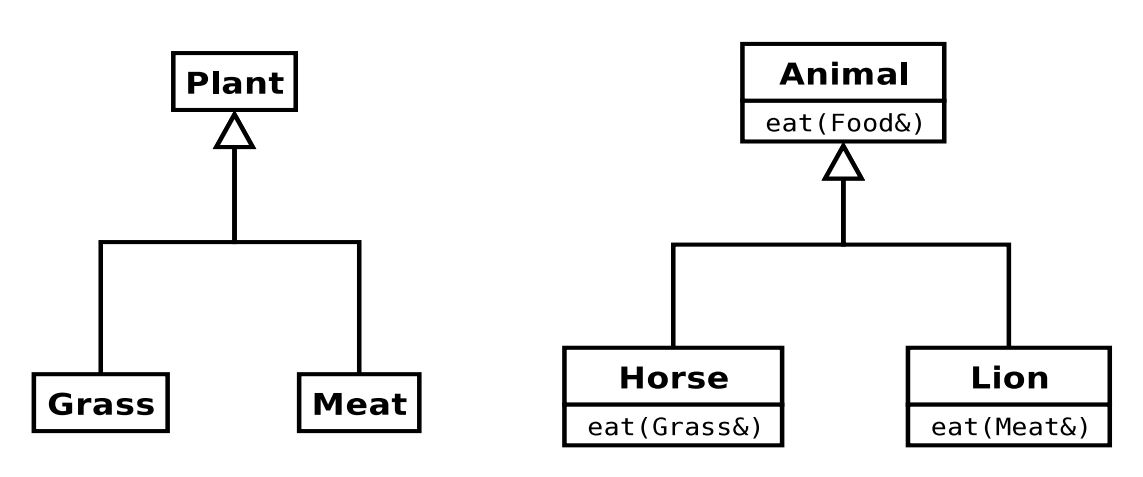
\includegraphics[width=0.7\linewidth]{familyPolymorphism}
		\label{fig:familypolymorhism}
	\end{figure}
	
	
	
	A probléma \lstinline[language=Eiffel]|Animal| osztály \lstinline[language=Eiffel]|eat()| feature-nél keletkezik. Különböző állatok különböző táplálékot igényelnek. Az oroszlánok csak húst esznek, míg a lovak csak növényeket.
	
	Különböző táplálék osztályok nem felcserélhetőek. A legtöbb objektumorientált nyelvben nem tudunk ilyesfajta megkötéseket tenni. (\href{http://icai.ektf.hu/pdf/ICAI2004-vol2-pp445-453.pdf}{link})
	
\subsection{ Milyen esetekben áll fenn altípus reláció paraméterezett típusok között az Eiffelben? Mit jelent itt a \lstinline[language=Eiffel]|frozen?|}
	Eiffelben (általában) a típusparaméter is kovariáns ha \lstinline[language=Eiffel]|class STACK[T]...|, akkor
	\begin{align*}
		STACK[INTEGER] <: STACK[ANY],
	\end{align*} de emiatt statikusan nem biztonságos a típusrendszer!

	Legyen $D[U]$ és $C[T]$ két paraméterezett típus. $D[U]<:C[T]$ akkor és csakis akkor állhat fenn, ha $D<:C$ és $U<:T$. (\href{https://www.eiffel.org/doc/eiffel/ET-_Inheritance#Polymorphism}{link})

	A \lstinline[language=Eiffel]|frozen| kulcsszót háromféleképpen használhatjuk. (\href{https://www.eiffel.org/doc/eiffel/Eiffel_programming_language_reserved_words#frozen}{link})
	
	Ha egy osztály header-jében alkalmazzuk expliciten a \lstinline[language=Eiffel]|frozen| kulcsszót, akkor ebből az osztályból nem lehet leszármaztatni.
	
	Ha egy feature deklarálásánál alkalmazzuk a \lstinline[language=Eiffel]|frozen| kulcsszót, akkor a feature-t nem lehet újradefiniálni egy leszármaztatott osztályban.
	
	Ha egy paraméterezett típus definiálásánál a típusparaméterre alkalmazzuk  a \lstinline[language=Eiffel]|frozen| kulcsszót, akkor a leszármaztatott paraméterezett típus csak ugyanazt a típus paramétert használhatja.
	
	Eiffelben (általában) a típusparaméter is kovariáns kivéve, ha \lstinline[language=Eiffel]|frozen| a típusparaméter, mert akkor invariáns. Ha \lstinline[language=Eiffel]|class STACK[frozen T] ...|, akkor nem áll fenn a következő összefüggés
	\begin{align*}
	STACK[INTEGER] <: STACK[ANY].
	\end{align*}
	
\subsection{ Mit jelent az attached (az Eiffel szabványban „!”) és a detachable (a szabványban „?”)? }
	Referencia típusok esetén a nullreferencia kérdése, illetve a nullable típusok természetesen Eiffelben is felmerülnek. A nullreferencia Eiffelben \lstinline[language=Eiffel]|Void| névre hallgat. A nullable vagy non-nullable tulajdonságok egy változó típusának meghatározásánál kapnak szerepet. A nullable Eiffelben \lstinline[language=Eiffel]|detachable|, míg a non-nullable \lstinline[language=Eiffel]|attached| kulcsszavakkal fejezhető ki. (\href{https://www.eiffel.org/doc/eiffel/Void-safety-_Background\%2C_definition\%2C_and_tools}{link})
	
	\begin{lstlisting}[language=Eiffel]
	my_attached_string: STRING
	my_detachable_string: detachable STRING
	
	...
	
	my_attached_string := my_detachable_string    -- Invalid
	my_detachable_string := my_attached_string    -- Valid
	\end{lstlisting}
	A fenti példában láthatjuk, hogy milyen módon feleltehetők meg egymásnak az \lstinline[language=Eiffel]|attached| és \lstinline[language=Eiffel]|detachable| változók, illetve, hogy alapvetően minden változó \lstinline[language=Eiffel]|attached|.
	
	Ha egy változó deklarációjában \lstinline[language=Eiffel]|attached| szerepel, akkor a fordító megakadályozza, hogy \lstinline[language=Eiffel]|Void| értéket kapjon, vagy bármi olyan értéket, amit \lstinline[language=Eiffel]|Void|-ra lehet állítani. (\href{http://www.ecma-international.org/publications/files/ECMA-ST/ECMA-367.pdf}{link} 8.11.1)

\subsection{ Milyen módon kezeli a kivételeket egy rutin, ha nincs benne rescue? }
	Eiffel-ben az \lstinline[language=Eiffel]|ANY| osztályban (minden felhasználói osztály ősosztályában) definiálva van egy \lstinline[language=Eiffel]|default_rescue| nevő metódus, melynek törzse alapértelmezésben csak egy üres utasítás. Ez az a feature, ami minden olyan esetben implicit módon meghívódik, amikor explicite nem adunk meg egy alprogram végén \lstinline[language=Eiffel]|rescue| részt, és az alprogram mőködése során mégis kivétel váltódik ki. Mivel minden felhasználói osztály az \lstinline[language=Eiffel]|ANY| class leszármazottja, ezért minden osztály felüldefiniálhatja ezt a metódust, saját igényei szerint. További öröklés esetén a felüldefiniált feature a leszármazottakra is érvényes lesz. Mivel Eiffel-ben a konstruktorok feladata az osztály-invariáns beállítása, ezért a \lstinline[language=Eiffel]|default_rescue|-t gyakran a paraméter nélküli konstruktor szinonímájaként szokták definiálni, hogy szervezett pánik esetén biztosítsa az invariáns visszaállítását. (\href{http://nyelvek.inf.elte.hu/leirasok/Eiffel/index.php?chapter=7}{link})

	\begin{lstlisting}[language=Eiffel]
		class C
		creation
			make, -- Other creation procedures if any ...
		inherit
			ANY
				redefine
					default_rescue
				end	
		feature
			make, default_rescue is
				-- No precondition
			do
				-- Appropriate implementation;
				-- Must ensure the invariant
			end -- make, default_rescue
			-- Other features ...
		end -- class C
	\end{lstlisting}

\subsection{ Mi a \lstinline[language=Eiffel]|default_create|? }
	Lehetőség van nem megadni \lstinline[language=Eiffel]|creation| klózt, ami azt jelenti, hogy a \lstinline[language=Eiffel]|default_create| alapvető creation procedure kerül meghívásra. A \lstinline[language=Eiffel]|default_create| az \lstinline[language=Eiffel]|ANY| osztályban kerül definiálásra, amit minden osztály örököl. Alapvetően egy üres utasítás.

	Eiffel-ben az objektumok dinamikusan rendelődnek hozzá a szimbólumokhoz. Lehetőség van konstruktorok megadására is. A nyelv alaptípusaihoz létezik automatikus kezdőérték hozzárendelés. Lokális változók esetén a kezdőérték hozzárendelés a rutin végrehajtása előtt történik meg, attribútumok esetén pedig az objektum létrehozásakor a konstruktor eljárás végrehajtása előtt. A kezdőértékek az egyes típusok esetén a következők,
	\begin{center}
		\begin{tabular}{|c|c|}\hline
			Típus																	& Érték\\\hline
			\lstinline[language=Eiffel]|INTEGER|     							   	& 0\\
			\lstinline[language=Eiffel]|REAL|, \lstinline[language=Eiffel]|DOUBLE| 	& 0.0\\
			\lstinline[language=Eiffel]|BOOLEAN|								   	& \lstinline[language=Eiffel]|false|\\
			\lstinline[language=Eiffel]|CHARACTER|	                               	& \lstinline[language=Eiffel]|null| karakter \\
			\lstinline[language=Eiffel]|BIT_N|										& csupa 0 bitsorozat\\
			Minden referencia típus 												& \lstinline[language=Eiffel]|Void|\\\hline
		\end{tabular}
	\end{center}
	
\subsection{ Hogyan szól a Liskov-féle helyettesítési elv (substitution principle)? }
	Minden osztály legyen helyettesíthető a leszármazott osztályával anélkül, hogy a program helyes működése megváltozna. Vagy pontosabban ha $B$ altípusa $A$-nek, akkor minden olyan helyen ahol $A$-t felhasználjuk $B$-t is minden gond nélkül behelyettesíthetjük anélkül, hogy a programrész tulajdonságai megváltoznának.
	
	Nézzünk egy egyszerű, ám annál híresebb példát: Kör-Ellipszis probléma:
	\begin{lstlisting}[language=C++]
	class Shape { }
	
	class Ellipse : Shape
	{
		public double MajorAxis { get; set; }
		public double MinorAxis { get; set; }
	}
	
	class Circle : Ellipse
	{
	
	}
	\end{lstlisting}
	
	Az osztályhierarchiában a Kör az Ellipszisből származik, lévén annak egy speciális esete. Na most, ha a fenti állításokat figyelembe vesszük, akkor egy rendkívül érdekes problémával nézünk szembe: tegyük fel, hogy egy olyan függvényt készítünk, amely egy ellipszis tengelyeit is módosítja. Ugye fönt kimondtuk, hogy ilyenkor ezt a függvényt bármely Kör objektumra is meghívhatjuk és most jön a lényeg: mi történik, ha egy Kör objektum tengelyei (az Ellipszisből származik, szóval nincs szigorúan vett sugár) megváltoznak?
	
	Azt bátran elmondhatjuk, hogy onnantól megszűnik Kör lenni, elméletileg legalábbis, de maga a Kör objektum – immár hibásan – még ugyanúgy létezik.
	
	Az elvet a következő szabályokon keresztül lehet betartani:
	\begin{itemize}
		\item Az előfeltétel a leszármazott osztályokban gyengíthetjük
		
		\item Az utófeltétel a leszármazott osztályokban erősíthetjük
	\end{itemize}
	
	Nézzük meg, hogy ez hogy működik a gyakorlatban! Térjünk vissza az eredeti Kör-Ellipszis példára, az Ellipszis osztály egy ki nem mondott előfeltétele, hogy a tengelyeket tetszés szerint módosíthatjuk. Ha a Kör osztályban megmondjuk, hogy ezt talán mégsem szeretnénk, azzal erősítjük az eredeti előfeltételt, vagyis a Kör osztályt ilyen módon nem használhatjuk Ellipszisként.

\subsection{Mi a kapcsolt (anchored) típus az Eiffelben? Mutass példát arra, hogy miért jó!}
	Lásd a \ref{like} kérdést!
	
\subsection{ Milyen szerződésnek kell eleget tegyen egy creation procedure? Írd le Hoare-hármas segítségével! }
	Lehetőség van megadni \lstinline[language=Eiffel]|creation| klózt. Alapvetően a \lstinline[language=Eiffel]|creation| klóz feladata az osztályinvariáns megteremtése.
	\begin{align*}
		\{Q_m\}make\{R_m\wedge inv_C\}
	\end{align*}
	ahol $make$ a creation procedure, $inv_C$ az osztály invariánsa, $Q_m$ és $R_m$ a creation procedure elő- és utófeltétele.
	
\subsection{ Mire való az \lstinline[language=Eiffel]|only| az Eiffelben (illetve a \lstinline[language=Eiffel]|strip| a jelenlegi implementációkban)? }
	Az \lstinline[language=Eiffel]|only| klóz szintaxisa a következő,
	\begin{align*}
	Only \triangleq \textcolor{RoyalBlue}{only} [Feature\_list]
	\end{align*}
	Az \lstinline[language=Eiffel]|only| klóz szintaxisából adódóan csak egy feature utókövetelményének legvégén szerepelhet.
	
	A többi utókövetelmény azt határozza meg, hogy a feature hogyan változtathat meg pár specifikus tulajdonságot, de lehetőség van azt is megadni, hogy miket nem változtat meg (ezt keret problémának nevezik - frame problem). Be tudjuk szűkíteni a feature hatását azzal, ha megkötjük melyik tulajdonságokat nem változtathatja meg.
	
	Egyik lehetőség, ha minden ilyen query-re definiálunk egy \lstinline[language=Eiffel]|q = old q| szabályt. Ez hosszú távon nem karbantartható, főleg, hogy a szülőosztályok megváltozásával újabb query-k kerülhetnek be.
	
	Erre nyújt megoldást az \lstinline[language=Eiffel]|only| klóz, amivel meg lehet kötni, hogy egy feature melyik query-ket változtatja meg. Azok a query-k, amik nincsenek felsorolva a feature nem változtathatja meg. Ez a megkötés nem csak az adott verzióra vonatkozik, hanem minden leszármazottra is.
	
	Az \lstinline[language=Eiffel]|only| klóz állhat üresen is, ekkor "tiszta" rutinról beszélhetünk, ami egyik query-t se változtatja meg.
	
	Egy $C$ osztálybeli \lstinline[language=Eiffel]|only| klóz akkor és csak akkor helyes, ha minden $q_n$ querry, ami megjelenik a feature listáján teljesíti a következőket,
	\begin{enumerate}
		\item $q_n$ csak egyszer fordul elő a feature listán
		\item $q_n$ a végleges neve a $C$ egy $q$ query-jének, argumentumok nélkül
		\item Ha $C$ újradeklarálja $f$-et egy $B$ szülőtől, akkor $q_n$ nem feature-e $B$-nek. 
	\end{enumerate}
	(\href{http://www.ecma-international.org/publications/files/ECMA-ST/ECMA-367.pdf}{link} 8.9.11)
	
	\lstinline[language=Eiffel]|only(x,y)| azt jelenti, hogy a \lstinline[language=Eiffel]|Current.x| és a \lstinline[language=Eiffel]|Current.y| megváltozhat a művelet hatására, de például a \lstinline[language=Eiffel]|Current.z| nem fog (ahol x, y és z az adott osztályban vagy bázisosztályaiban deklarált query-k). A jelenlegi implementációban ezt úgy írhatjuk, hogy \lstinline[language=Eiffel]|equals(strip(x,y), old strip(x,y))|, ahol a \lstinline[language=Eiffel]|strip| segítségével projektálhatjuk a \lstinline[language=Eiffel]|Currentet| a megnevezett mezőkre, az \lstinline[language=Eiffel]|old| segítségével pedig a műveletbe való belépés pillanatában érvényes értékre hivatkozhatunk. Az objektum belső állapotát meg nem változtató műveleteket only()-val jelölhetjük.
	
\subsection{ Mi a különbség a strukturális és a nominális altípusosság között? }
	Strukturális altípusosság esetén a felépítés alapján hasonlítunk össze két típust. Két típus egyenlő, ha ugyanaz a struktúrális felépítésük (pl. ugyanazokat a feature-öket tartalmazzák). Egy $A$ típus altípusa $B$-nek, ha minden résztípusa altípusa a megfeleltetésének $B$-ben (pl. függvényeknél kontravariáns argumentumok). “Típusok felépítése szerinti induktív definíció”. Ezzel olyan típusok is relációba kerülhetnek, amelyeknek “nem kellene”.
	
	Nominális altípusosság esetén a név alapján hasonlítunk össze két típust. Ilyen módszerrel két típus ugyanaz, ha a nevük megegyezik. Egy típus akkor altípusa a másiknak, ha ezt explicit kimondtuk (pl. \lstinline[language=Eiffel]|inherit|, \lstinline[language=Java]|extends|, stb.).
	
\subsection{ Mit jelent a polymorphic CAT-call? }
	A CAT jelentése Changed Availability or Type.
	
	CAT-call-nak nevezzük egy $B$ osztály $f$ feature-ére vonatkozó hívást a $C$ osztályban, ha $D<:B$ esetén a következők közül bármelyik fennáll, ahol $D$ nem a \lstinline[language=Eiffel]|NONE|.
	\begin{itemize}
		\item $D$ megváltoztatja a láthatóságát $f$-nek úgy, hogy $C$ ne érje el.
		\item $D$ redeclares $f$ such that the call's actual argument signature does not conform to the redeclared formal argument signature.
		\item The version of $f$ in $D$ has a formal argument of a type anchored either to \lstinline[language=Eiffel]|Current| or to a feature that $D$ redeclares to a type to which the corresponding actual argument's type does not conform.
	\end{itemize}

	A CAT-call egy futási idejű próbálkozás arra vonatkozóan, hogy végrehajtsunk egy olyan hívást, ami nem hajtható végre az adott elemen.
	
	A típus rendszer feladata, hogy biztosítsa, hogy egy helyes rendszer végrehajtása során soha ne történjen CAT-call.
	
	A CAT egy rövidítés “Changed Availability or Type”, ami két nyelvi mechanizmust kapcsol össze, melyeket ha a típus rendszer nem kezel megfelelően, CAT-call történhet.(\href{http://www.ecma-international.org/publications/files/ECMA-ST/ECMA-367.pdf}{link} 8.25.1)
	
\subsection{ Mit értünk az alatt, ha egy objektumművelet esetén a paraméterek nonvariánsak? Milyen problémát vet fel? }
	Invariánsak vagy nonvariánsak a paraméterek, ha se nem kovariánsak se nem kontravariánsak.	
	
\subsection{ Hogyan, milyen módokon örökölheti meg az $A$ osztály a $B$ osztály egy $f$ feature-ét, ha $C$ és $D$ a $B$ gyermeke, valamint $A$ a $C$ és a $D$ gyermeke? Milyen eseteket különböztethetünk meg? }

	Ez egy többször öröklés egy őstől.
	
	\begin{itemize}
		\item Ha egyik osztályban sincs implementáció, akkor $A$-ban implementálható $f$.
		\item Ha $C$ és $D$ is implementálja $f$-et, de azonos módon, akkor \lstinline[language=Eiffel]|join|-olhatóak.
		\item Ha $C$ és $D$ is implementálja $f$-et, de eltérő módon, akkor \lstinline[language=Eiffel]|undefine| és \lstinline[language=Eiffel]|redefine| alkalmazhatóak.
		\item Ha $C$ és $D$ is implementálja $f$-et más-más néven, akkor mindkét feature-t megörököljük. Lehetséges, hogy szükség lesz \lstinline[language=Eiffel]|select|
	\end{itemize}
	
\subsection{ Milyen lehetőségeket biztosít egy kovariáns sablonparaméter? }
	$List[D] <: List[B]$, ha $D<:B$. Innentől már ki lehet használni az altípusos polimorfizmust.
	
\subsection{ Mi a név szerepe, és miért fontos az átnevezés az Eiffelben? }
	A névvel tudunk azonosítani egy objektumot, feature-t. 
	
	Átnevezés szükséges lehet többszörös/ismételt öröklődés használatakor. Ennek segítségével elérhetővé válhat több azonos nevű, de eltérő implementációjú leszármaztatott feature, ha mindegyiket más nevet kap.
	
\subsection{ Mi a különbség a nyilvános és a privát öröklődés között? }
	Privát öröklődés esetén csak az adott osztály tudja használni a privátan megörökölt metódusokat. A megörökölt metódusok nem lesznek exportálva.
	
	Publikus öröklődés esetén mindenki tudja hívni az osztályon a publikusan megörökölt metódusokat. Az öröklött metódusok export státusza az ősosztályban lévővel lesznek egyenlőek.
	
\subsection{ Milyen problémákat vet fel a többszörös öröklődés? }
	Az első legszembetűnőbb probléma a névütközés, melyre az egyik megoldást a \ref{atnevezes} kérdés szolgáltatja. Másik lehetőség ha az \lstinline[language=Eiffel]|undefine| kulcsszóval töröljük az egyik őstől származó member-t.
	
	A másik probléma amit felvet a többszörös öröklődés a gyémánt alakú öröklődés. Ennek feloldásában a mixinek segíthetnek, melyet a \ref{Mixin} kérdés tárgyal. 
	
\subsection{ Mik az expandált típusok? }
	\lstinline[language=Eiffel]|expanded Class exp ...| egy expandált osztály definíció. Olyan típusok, amelyekből a létrehozott példányok nem egy objektumra mutató referenciák lesznek, hanem tényleges objektumok. Tehát bármelyik \lstinline[language=Eiffel]|exp| típusú változó az \lstinline[language=Eiffel]|exp| osztály egy példányát fogja tartalmazni. Szemben egy sima osztállyal, amikor a változó csak egy referenciát tartalmaz a tényleges objektumra. Ez megmutatkozik az értékadások esetén, vagy a paraméterátadásnál, ahol expandált típusok esetén másolás történik, nem expandáltaknál pedig csak referenciák átállítása.
	
\subsection{ Hogyan számoljuk ki egy osztály invariánsát? (. . . öröklődés . . . ) }
	Az \lstinline[language=Eiffel]|invariant| klózban megfogalmazott feltételek illetve a szülőosztályok invariánsainak konjunkciójaként.

\subsection{ Mit értünk sekély, illetve mély másoláson? }
	A sekély másolás (shallow copy) célja, hogy minél kevesebbet másoljon. A referenciákat csak lemásolja, és nem duplikálja a HEAP-en lévő objektumokat.
	A másolt és az eredeti referencia aliasként működnek ugyanarra a HEAP területre.
	
	A mély másolás (deep copy) lényege, hogy a referenciák által hivatkozott értékeket is lemásolják, és a másolt referenciák ezekre fognak mutatni.

\subsection{ Milyen lehetőségek vannak a referenciák nem-ürességének leírására az Eiffelben? }
	Referencia típusok esetén közvetlenül ráellenőrizhetünk, hogy az adott változó nem nullreferencia-e.
	\begin{lstlisting}[language=Eiffel]
		if x /= Void then
			-- Any other instructions here that do not assign to x
			x.f (a)
		end
	\end{lstlisting} 
	
	Referencia típusok esetén használhatjuk az \lstinline[language=Eiffel]|attached| kulcsszót.
	\begin{lstlisting}[language=Eiffel]
		if attached x as l_x then
			l_x.f(a)
		end
	\end{lstlisting}
	
	 A változó deklarációjánál kiköthetjük, hogy soha nem kaphat értékül nullreferenciát (fordítási idejű hibát okoz).
	\begin{lstlisting}[language=Eiffel]
		my_attached_string: attached STRING
	\end{lstlisting}
	
\subsection{ Mi az $F$-bounded polimorfizmus? Mutass rá példát Javában! }
	A bounded polimorfizmust eredetileg a $System_{F<:}$ leírásánál tanulmányozták, de elérhető modern objektumorientált nyelvek (Java, C\#, Scala) esetében, mint paraméteres polimorfizmus (template-ek). 
	
	Az F-bounded polimorfizmus vagy rekurzív bounded polimorfizmus sokkal pontosabb típusozásra ad lehetőséget rekurzív típusokat alkalmazó függvények esetében. Egy rekurzív típus definiál egy olyan függvényt, ami vagy paraméterében vagy visszatérési értékében hivatkozik a típusra.
	
	Legyen adott egy \lstinline[language=Java]|Moveable| osztály, melyet egy \lstinline[language=Java]|moveMeOneInch| függvénnyel el lehet mozdítani egy inch-csel.
	\begin{lstlisting}[language=Java]
		Moveable {
		Moveable move(int x, int y)
		}
		
		Moveable moveMeOneInch(Moveable m) {...}
	\end{lstlisting}
	
	\lstinline[language=Java]|moveMeOneInch| működni fog az \lstinline[language=Java]|Car|, \lstinline[language=Java]|Trains|, \lstinline[language=Java]|Points| osztályokon és mindenen olyan osztályon, ami \lstinline[language=Java]|Moveable|. Ezzel minden rendben lenne, de a visszatérési értéket cast-olni kell.
	\begin{lstlisting}[language=Java]
		Car c = ...
		Car movedCar = (Car) moveMeOneInch(c);
	\end{lstlisting}
	De Java 5 óta írhatjuk a következő F-bounded polimorfizmust.
	\begin{lstlisting}[language=Java]
		<T extends Moveable> T moveMeOneInch(T m) {...}
		
		Car c = ...
		Airplane p = ...
		
		Car movedCar = moveMeOneInch(c);
		Airplane movedAirplane = moveMeOneInch(p);
	\end{lstlisting}
	Itt már típus helyes lesz a visszatérési érték.
	
\subsection{ Mit jelent a “frame condition” kifejezés? Hogyan írunk ilyet az Eiffelben? }
	Megszorítások a változókra. Ez az \lstinline[language=Eiffel]|only| vagy a \lstinline[language=Eiffel]|strip| segítségével tehető meg.
	
\subsection{ Milyen kifejezések szerepelhetnek értékadás baloldalán az Eiffelben? }
	Csak írható entitások (változók) állhatnak egy értékadás baloldalán. Ez által a függvényparaméterek például nem szerepelhetnek értékadás bal oldalán, se az osztály memberjei sem.
	\lstinline[language=Eiffel]|obj.some_attribute := some_value| nem valid utasítás.
	
	A member-eket csak metódusokkal vagy úgy nevezett \textit{assigner command} definiálásával lehet módosítani. \textit{Assigner command} használatával a fenti értékadás már lehetséges.
	\begin{lstlisting}[language=Eiffel]
		some_attribute: SOME_TYPE assign set_some_attribute
	\end{lstlisting}
	Ezzel automatikusan definiálunk egy setter-t a member-hez.
	
\subsection{ Mire jó a \lstinline[language=Eiffel]|debug| utasítás az Eiffelben? }
	A \lstinline[language=Eiffel]|debug| szintaxisa a következő,
	\begin{align*}
	Debug \triangleq \textcolor{RoyalBlue}{debug} [ "("Key\_list ")" ] Compound\; end
	\end{align*}
	
	Az Eiffel támogatja a debug-olást. Ehhez megadhatjuk globálisan vagy egyesével, hogy mely \lstinline[language=Eiffel]|Key_list|-beli elemek legyenek aktívak, vagyis az ezekre vonatkozó \lstinline[language=Eiffel]|Compaund| klóz végrehajtódnak.
	
	\begin{lstlisting}[language=Eiffel]
		debug("MY_DEBUG_FLAG")
			-- Debug code is here.
		end
	\end{lstlisting}
	A fenti kódrészlet megfelel a C-ben megszokott kódrészleteknek.
	\begin{lstlisting}[language=C]
	#ifdef MY_DEBUG_FLAG
		/* Debug code is here */
	#endif
	\end{lstlisting}
	
\subsection{ Hogyan történik a paraméterátadás az Eiffelben? Térj ki az expandált típusokra is! }
	Általános esetben, nem expandált típusok esetén referencia szerinti paraméterátadás történik, azaz nem másolódik maga a bemeneti paraméter, csak egy referenciát kapunk rá, de ezt nem állíthatjuk át. Viszont műveleteket hívhatunk a paraméterként kapott objektumon.
	
	Expandált típusok esetében, mivel ezek stack-allokált objektumok, így amikor egy ilyen típust adunk át, akkor érték szerinti paraméterátadás történik, azaz másolódik.
	
\subsection{ Milyen elvárások fogalmazhatók meg egy egyenlőségvizsgálat műveletre? }
	Matematikai értelemben egy egyenlőség reláció reflexív (1), szimmetrikus (2), tranzitív (3)
	\begin{align}
	x=x\\
	x=y\implies y=x\\
	x=y \wedge y=z\implies x=z
	\end{align}
	 
	Ha $A$ és $B$ különböző típusú, akkor nem lehetnek egyenlőek.
	
	Ha $A$ és $B$ megegyező típusúak, akkor implementáció függő lehet az egyenlőség. A strukturális egyenlőség azt várja el, hogy a két objektum ugyanolyan tartalmú legyen. A referenciális egyenlőségnek csak annyi a feltétele, hogy azonos elemre mutasson a két referencia.
	
\subsection{ Mi a különbség egy exportált és egy nem exportált feature szerződésében? Mutasd be Hoare-hármas segítségével! }
	Egy exportált $r$ feature esetében az osztálynak kívülről konzisztensnek kell maradnia, vagyis az osztály invariánst meg kell tartani
	\begin{align*}
		\{ Q_r \wedge inv_C \}r\{ R_r \wedge inv_C \},
	\end{align*}
	ahol $Q_r$ és $R_r$ az $r$ feature elő- és utófeltétele, míg $inv_C$ az osztályinvariáns.
	
	Egy nem exportált $r$ feature nem elérhető az osztályon kívülről, így ennek nem kell az invariánst megtartania.
	\begin{align*}
	\{Q_r\}r\{R_r\},
	\end{align*}
	ahol $Q_r$ és $R_r$ az $r$ feature elő- és utófeltétele.
	
	Érdemes figyelni, hogy egy exportált metódus nem feltétlenül használható rögtön nem-exportáltként, hiszen a meghívása előtt az osztályinvariánst garantálni kell, míg nem-exportált esetben ez nem szükséges.
	
\subsection{ Mit értünk multimethodon? }
	Bizonyos objektumorientált nyelvekben a dinamikus kötés nem egyetlen kitüntetett paraméter dinamikus típusán működik, hanem az összes paraméter dinamikus típusát figyelembe veszi. Például az Eiffelben az \lstinline[language=Eiffel]|a.b(c)| rutinhívásnál az \lstinline[language=Eiffel]|a| és a \lstinline[language=Eiffel]|c| változók statikus típusa alapján dől el, hogy a \lstinline[language=Eiffel]|b| rutin hívása értelmes-e, és az \lstinline[language=Eiffel]|a| változó dinamikus típusa alapján dől el, hogy a művelet mely osztályban definiált implementációja hajtódik végre. Egy \textit{multimethodokat} (azaz multiple dispatchet) támogató nyelvben az \lstinline[language=Eiffel]|a| és a \lstinline[language=Eiffel]|c| dinamikus típusa alapján választódik ki a végrehajtandó kód (azaz az a statikus típusában, illetve leszármazottaiban több olyan \lstinline[language=Eiffel]|b| művelet is lehet, amelynek a paramétere a \lstinline[language=Eiffel]|c| statikus típusának valamilyen altípusába tartozik).
	
	A multimethodokat támogató nyelvekben az úgynevezett bináris műveletek (azaz amikor a művelet paraméterének típusa a fogadó objektum típusával kell megegyezzen, mint mondjuk egyenlőségvizsgálatnál) megvalósítása megoldott, hiszen minden osztályban megírhatjuk az arra az osztályra jellemző (és a fogadó és paraméter objektumot ugyanazzal típusozó) implementációt, és a dispatch során a legjobban illeszkedő implementáció hívódik meg. A szimmetriáról a multiple dispatch gondoskodik.

\subsection{ Mik a virtuális típusok? Mire jók? }
	Alternatíva a típusparaméterekre. Az ősosztályban a típusparaméterek, mint tagok vannak deklarálva, és az absztrakt alosztályokban lehet specializálni őket. A konkrét alosztályban meg kell mondani, hogy ezek a típusok mit jelentenek.
	
\subsection{ Mit nevezünk parametrikus polimorfizmusnak? }
	Általános viselkedés leírása típusparaméterek segítségével. Így az általános kód különböző konkrét típusokra is képes a működésre.
	\begin{lstlisting}[language=C]
	class List<A> {   ...   }
	List<Integer> integerList;
	List<String>  stringList ;
	\end{lstlisting}
	
\subsection{ Mit nevezünk altípusos polimorfizmusnak? }
	A Liskov-féle helyettesítési elv szerint, ha $B <: A$, akkor az $B$ típusú objektumok használhatóak úgy, mintha $A$ típusúak lennének.
	\begin{lstlisting}[language=Java]
	class Animal {}
	class Dog extends Animal {}
	class Cat extends Animal {}
	
	void foo(Animal a) {}
	
	foo(new Dog())
	foo(new Cat())
	foo(new Animal())
	\end{lstlisting}
